\chapter{MapD}

\begin{wrapfigure}{r}{0.2\textwidth}
  \begin{center}
    
\includegraphics[width=100pt]{images/mapd_logo.png}
  \end{center}
  \caption[MapD]{MapD Logo}
\end{wrapfigure}


MapD is a GPU database with the goal to speed up queries and analytic tasks with the power of GPU's
and their massive parallel architectures consisting of thousands of cores.
The first prototype of MapD was develop in 2012 by Todd Mostak.
A year leater MapD was incubated at the  MIT’s Computer Science and Artificial Intelligence Laboratory (CSAIL) database group
and in September 2013 Todd Mostak founded MapD Technologies, Inc.
They have got two products called MapD Core \cite{mapdcore} and MapD Immerse \cite{immerse}.
The MapD Core SQL engine is an open source in-memory, SQL, GPU database and
MapD Immerse is a tool for visual analytics on top of MapD Core SQL engine.


\begin{figure}[H]
    \centering
    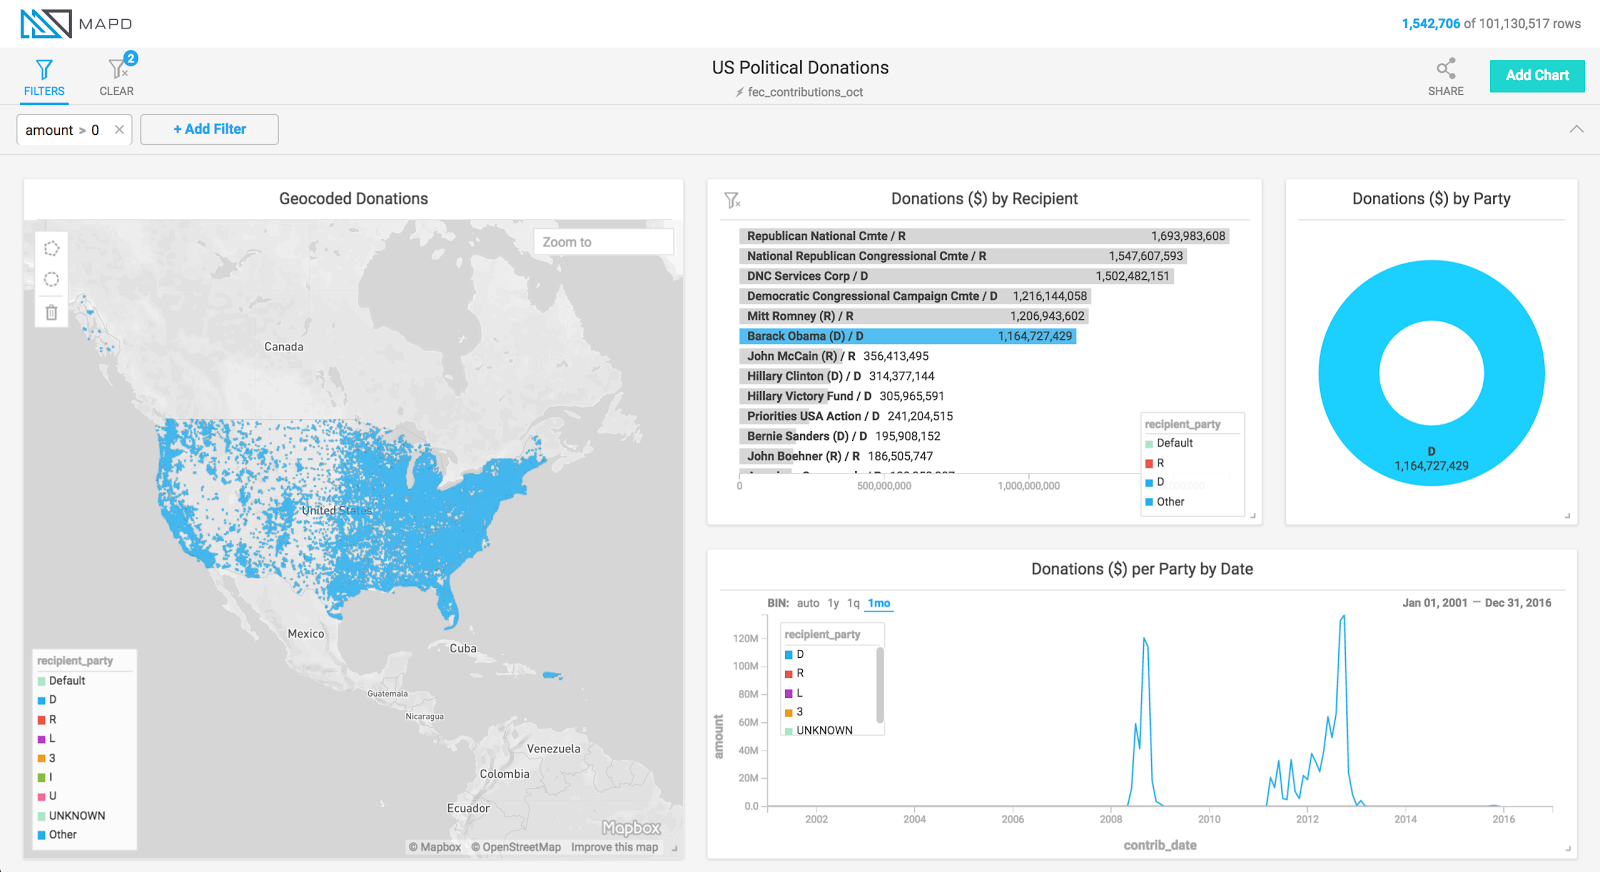
\includegraphics[width=0.9\textwidth,height=0.9\textheight,keepaspectratio]{images/mapd_imerse.png}
    \caption{MapD Immerse \cite{filtering}}
    \label{fig:immerse}
\end{figure}


\newpage
\subsection{Functional Properties}
Related to the excellent Survey of Sebastian Bress et al. \cite{bress2014gpu} MapD has the following functional properties.

\subsubsection{Storage system} MapD has got a relational DBMS that is able to handle data amounts bigger than the memory space.
But tries to hold as much data as possible in-memory to to improve the performance.
\subsubsection{Storage model} MapD uses a columnar layout to store the data and uses so called chunks, which split the columns in smaller pieces.
The chunks are the basic units of the memory manager.
\paragraph{Processing model} MapD processes on operator-at-a-time or one chunk per operation. Thus it is a block-oriented processing.
The queries are compiled for the CPU and the GPU.
\subsubsection{Query processing}
\paragraph{Query placement} In contrast to \cite{bress2014gpu} the gained experience with MapD showed that MapD tries to run the queries on the GPU even if there isn't enough space and isn't able to handle such queries on his own.
Hence the user has to switch the execution mode from GPU to CPU.
\paragraph{Optimization} MapD's optimizer tries to execute the queries on the most suitable device, like text searching using an index on the CPU and table scans on the GPU.
\subsubsection{Transactions support} MapD doesn't not support transactions and doesn't support UPDATE or DELETE operations on the inserted data, either.
That could be related to the difficult task of handling persistence between the CPU and GPU or even distributed systems at all.


\newpage
\section{Overview}

The following section will give you an overview about the handling of MapD.
Often there will be a comparison between MapD and PostgreSQL to point out the differences and similarities of these two databases.



\subsection{Data Definition Language (DDL)}
The DDL seams familiar since it uses SQL syntax \cite{ddl}.
The syntax to handle users, databases, tables, and views is listed below.

\paragraph{User}
\begin{itemize}
 \item CREATE USER
 \item DROP USER
 \item ALTER USER
\end{itemize}

\paragraph{Database}
\begin{itemize}
 \item CREATE DATABASE
 \item DROP DATABASE
\end{itemize}


\paragraph{Table}
\begin{itemize}
 \item CREATE TABLE
 \item CREATE TABLE AS SELECT
 \item ALTER TABLE
 \item DROP TABLE
 \item TRUNCATE TABLE
\end{itemize}

\paragraph{View}
\begin{itemize}
 \item CREATE VIEW
 \item DROP VIEW
\end{itemize}


\subsubsection{Datatypes}
MapD supports the data types shown in table \ref{tab:datatypes}.
To get a better intuition the corresponding PostgreSQL data types are listed as well.

\begin{table}[H]
\centering
\begin{tabular}{ |l|l|l|l| }
\hline
\multicolumn{2}{| l |}{MapD} & \multicolumn{2}{| l |}{PostgreSQL}  \\
\hline
Data type & Size [bytes] & Data type & Size [bytes]  \\
\hline
TEXT & Variable & text & Variable \\
TIMESTAMP	& 8 & timestamp & 8 \\
TIME	& 8 & time & 8 \\
DATE	& 8 & date &  4 \\
FLOAT	& 4 & real & 4 \\
DOUBLE	& 8 & double precision & 8 \\
INTEGER	& 4 & integer & 4 \\
SMALLINT & 2 & smallint & 2 \\
BIGINT	& 8 & bigint & 8 \\
BOOLEAN	& 1 & boolean & 1 \\
DECIMAL	& 8 & numeric & variable \\
\hline
\end{tabular}
\caption{Data types \cite{mapddatatype} \cite{postgresdatatype}}
\label{tab:datatypes}
\end{table}

As you can see MapD supports the common data types.
And if you compare them to the corresponding PostgreSQL types they have got nearly the same names.
In addition PostgreSQL provides further data types like json or box which allow extended possibilities of use.


\subsection{Data Manipulation Language (DML)}
As well as the DDL of MapD the DML uses the SQL syntax too.
MapD currently supports the instructions:
\begin{itemize}
 \item INSERT INTO
 \item SELECT
\end{itemize}

Until now there is no support for the operations:
\begin{itemize}
 \item DELETE
 \item UPDATE
\end{itemize}
But they are in development, since MapD don't want to compromising the speed much with these instructions it may take a while.

Furthermore, MapD provides operations like EXPLAIN, LIKELY/UNLIKELY, Aggregate Functions and Conditional Expressions to improve the DML operations and extend the functionality.

\subsection{Data import}
MapD allows to import data from different sources as you can see in the following section.

\subsubsection{COPY FROM}
The COPY FROM operation is callable from the mapdql terminal and imports data from a local CSV or related format file into the database.

\subsubsection{SQL Importer}
The SQL Importer is a java tool that allows to run queries on other database via JDBC and stores the results in to MapD.

\subsubsection{StreamInsert}
The StreamInsert program could be attached at the end of a real-time stream processing engine like Kafka or a similar product to import stream data into MapD for further analytic tasks.

\subsubsection{HDFS}
The tool sqoop-export offers the possibility to import CSV or Parquet files from a HDFS file system into MapD database.

\subsection{Data export}
To export data from MapD, mapdql provides the command COPY TO that allows to export the result of a SELECT statement to a file.
For example like:
\begin{itemize}
 \item COPY (SELECT * FROM tweets) TO '/tmp/tweets.csv';
\end{itemize}


\newpage
\subsection{Client interfaces}
MapD provides a tool called mapdql \cite{mapdql} as a client-side SQL console that displays query results you submit to the MapD Core Server.
The counterpart of PostgreSQL is psql \cite{psql}.

\subsubsection{Database connection}
To following commands compares the connection to MapD respectively PostgreSQL with mapdql and psql.
\begin{itemize}[noitemsep]
 \item[mapdql:]  mapdql <database>  -u <user> -p <password> --port <port> -s <host>
 \item[pgsql:]  psql -h <host> -p <port> -U <user> -W <password> <database>
\end{itemize}

\subsubsection{Commands}
The table \ref{tab:commands} lists some basic commands of mapdql and pgsql.
It is only a slight slice of all possible commands, but another good example to point out how much in common those two products have.
\begin{table}[H]
\centering
\begin{tabular}{ |l|l|l| }
\hline
Command & mapdql & pgsql  \\
\hline
	List databases & \textbackslash l &  \textbackslash l \\
	List tables in database & \textbackslash t &  \textbackslash d \\
	Describe a table & \textbackslash d <table> & \textbackslash t <table> \\
	Connect to a database &  \textbackslash c  & \textbackslash c \\
	Print timing information & \textbackslash timing & \textbackslash timing \\
	Switch to GPU mode & \textbackslash gpu & - \\
	Switch to CPU mode & \textbackslash cpu & - \\
	Quit & \textbackslash q & \textbackslash q \\
\hline
\end{tabular}
\caption{Commands}
\label{tab:commands}
\end{table}

\subsubsection{Alternative interfaces}
Beside of mapdql MapD provides the following interfaces:
\begin{itemize}
 \item JDBC
 \item ODBC
 \item pymapd
 \item Python JayDeBeApi
 \item SQuirreL SQL
 \item RJDBC
 \item Apache Thrift
\end{itemize}